% Code review of RCB
\documentclass[11pt,a4paper]{article}
\usepackage{graphicx, pdfpages}
\title{Ram Control Block Code Review}
\author{Jonathan Ely}

\begin{document}
\maketitle
\section{

\section{Compilation}
Farhan's files compile with no warnings or errors in Modelsim, with
the compilation set to 1993 VHDL and 'Check for Synthesis enabled'.

\section{Synthesis}
Despite Modelsim showing now complaints, Synplify did come up with a 
couple of errors and warnings. 

\subsection{Errors}
The errors all related to the declaration
of the \emph{pix_write_cache} instance in \emph{rcb.vhd}. Here, Farhan
forgets to map the \emph{w_size} and \emph{p_size} generics causing width
errors since the \emph{w_size} and \emph{p_size} generics decared in 
\emph{pix_write_cache.vhd} are not the same size as those used in \emph{rcd.vhd}.

\subsection{Warnings}
Synplify displays two warnings from the \emph{rcb.vhd} file.

The first is regarding the OTHERS section of the nextstate CASE statement on line 198.
Synplify states \"Others clause is not synthesised\", this is because there
are no other states - all the states in the enumerated type have been accounted for.

The last warning is due to an undriven signal in \emph{rcb.vhd}. \emph{delaycmd1}
is not driven at at any point, however it is read from in several IF statements. 
It seems the purpose of this signal is to be able to read the \emph{delaycmd} signal
since VHDL does not allow the reading of an output. To fix this warning line 211 
should be changed to drive \emph{delaycmd1}.

\section{FSMs}
Farhan's FSM appears to work and the selection of states is sensible.

\section{Reset}


\section{Code Correctness}


\section{Design Correctness}


\section{Code Style}
On the whole Farhan's code is fairly clear and well writen. However it would be 
nice if there were more comments.

%include Farhan's Documentation
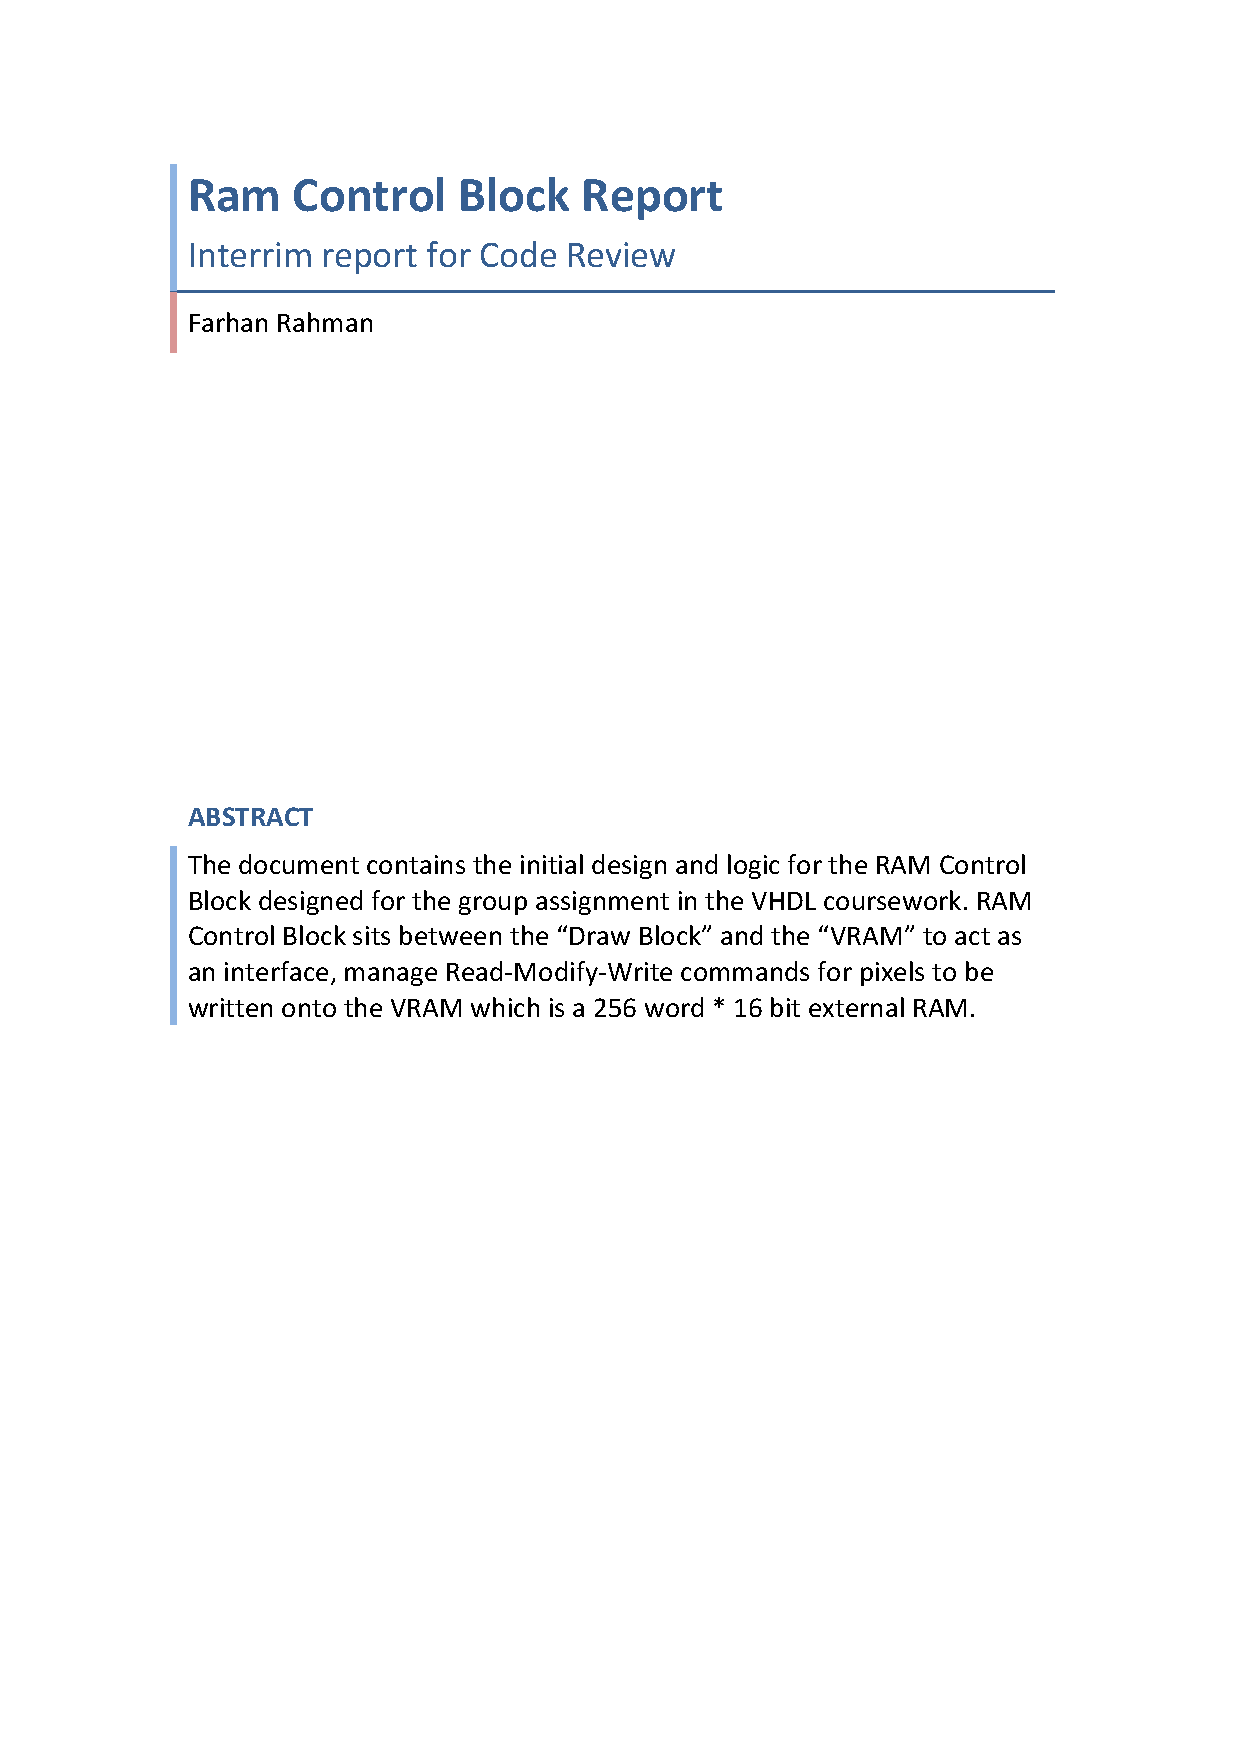
\includepdf[pages=-]{RCBDocumentation.pdf}
\end{document}
